%!TEX root = main.tex

\subsection{Datasets}
\label{sec:dataset}

% \subsection{Data description}
% \label{sub:data-des}

% The four TCP connections of the front-end server use different port number to distinguish each other. We use tcpdump to collect the TCP traces of all the four connections in one front-end relay server. Our collection span from July 15, 2015 to July 22, 2015, totally 7 days, 24 hours each day. 

The packet-level dataset we use for analysis was collected via tcpdump in one front-end server, which spans from Jul 15th, 2015 to Jul 22nd 2015. Overall, we collected 4.88 billion packets, corresponding to 1.24 million flows. The average packet size is 1028 bytes and average flow size is 3.86MB. Through examining the TCP ports that each packet is assigned, we could distinguish which one of the four connections (flows) the packet belongs. 

Figure~\ref{fig:use-fre} shows the variation of the amount of user upload and download over one week. In the figure, we observe that the number of download flows is much larger than that of upload flows, which means that more users view videos instead of sharing their videos. Users sharing or viewing videos follows similar diurnal pattern across the week. For both of upload and download flows, the number of access continues to grow from 6AM and reaches peak at 11PM. In the weekly pattern, the number of download flows reaches peak of the week in the evening of Saturday. It is easy to understand as most people use the crowdsourced live video as a kind of entertainment and do not use it in work time.

\begin{figure}[t]
\centering
\subfloat[Number of users' upload and download flows.]{
	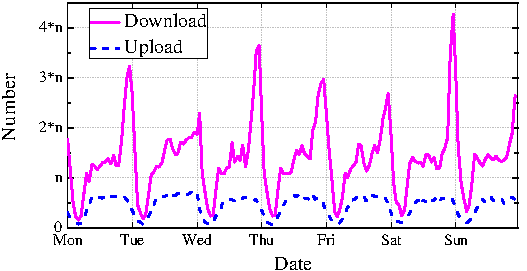
\includegraphics[width=2.5in]{use-fre}
	\label{fig:use-fre}}
\hspace{1em}%
\subfloat[Upload and download flows' complete time.]{
	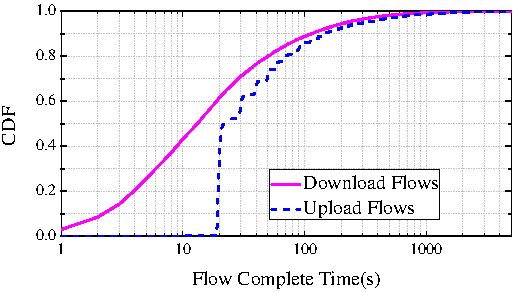
\includegraphics[width=2.5in]{flow-time}
	\label{fig:flow-time}}
	\hspace{1em}%
\subfloat[Upload and download flows' size.]{
	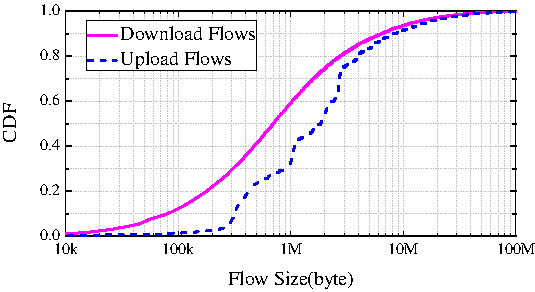
\includegraphics[width=2.5in]{flow-size}
	\label{fig:flow-size}}
\subfloat[The rate of upload and download flow.]{
	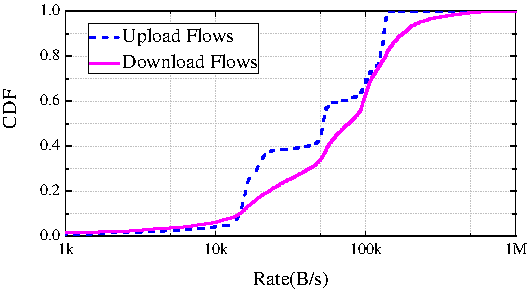
\includegraphics[width=2.5in]{rate}
	\label{fig:flow-rate}}
\caption{Dataset  description.}%
\label{fig:dataset} %% label for entire figure
\termspace
\end{figure}

Figure~\ref{fig:flow-time} shows the distribution of complete time of both upload and download flows. For the download flows, we define the \emph{flow complete time} as the interval between the front-end server receives the first SYN packet and it receives the acknowledgment of the last byte of data. For upload flows, the \emph{flow complete time} is defined as the interval between the front-end server receives the first SYN packet and it receives the last byte of data from the client. In upload flows, the servers will send keep-alive packet when idle and terminate the flows if it can not receive any data from client in 20 seconds. That is why there are nearly no upload flows with completion time less than 20s. For both upload and download flows, about 60\% of flows are less than 30s. It indicates that most of users view or share short videos. As some users may terminate to view the video while the video sharing users may continue to upload video, the flow complete time of upload flows is longer than that of download flows.   

%\begin{figure}[ht]
%	\centering
%	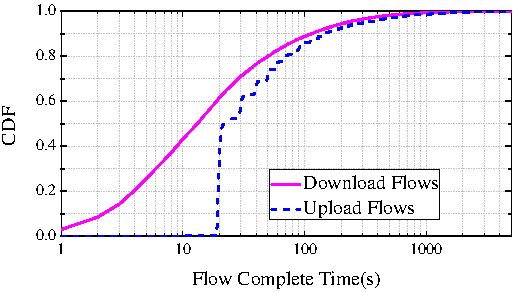
\includegraphics[width=\linewidth]{flow-time}
%	\caption{Upload and download flow complete time.}
%	\label{fig:flow-time}
%	\termspace
%\end{figure}

Figure~\ref{fig:flow-size} shows the distribution of flow size, defined as the amount of transmitted data bytes, for both upload and download flows. About 60\% of download flows and 40\% of upload flows are less than 1MB, which means most of crowdsourced live videos are short. In Figure~\ref{fig:flow-size}, we can also see that download flows are smaller than upload flows, the same with the flow complete time.

%\begin{figure}[ht]
%	\centering
%	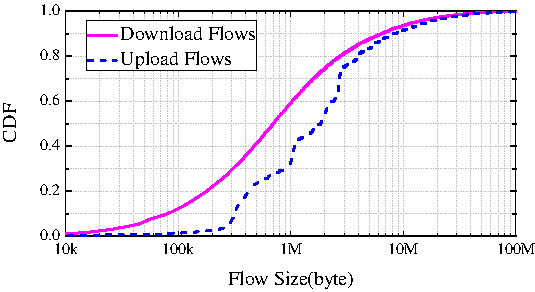
\includegraphics[width=\linewidth]{flow-size}
%	\caption{Upload and download flows size.}
%	\label{fig:flow-size}
%	\termspace
%\end{figure}

Figure~\ref{fig:flow-rate} shows the distribution of throughput of upload and download flows. From the figure we can see that the throughput of upload flows is smaller than that of download flows, which could be explained as follows. First, in most networks, upload bandwidth is smaller than download bandwidth (\eg the upload bandwidth of ADSL(Asymmetric Digital Subscriber Loop) is 640Kbps while the download bandwidth is 6-8Mbps~\cite{wei2008classification}). Second, as video is fetched from the storage server without waiting in download flows while in upload flows video data can only be transmitted when cameras produce video data. 
%\begin{figure}[ht]
%	\centering
%	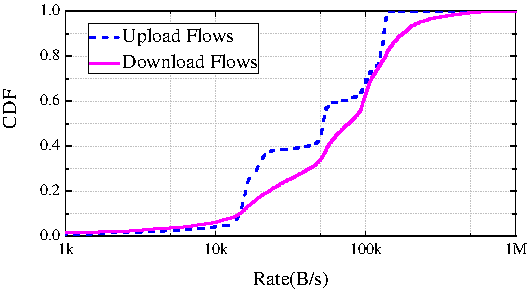
\includegraphics[width=\linewidth]{rate}
%	\caption{The rate of upload and download flow.}
%	\label{fig:flow-rate}
%	\termspace
%\end{figure}
